\chapter{Tabela de Dispersão}

No capítulo anterior, apresentamos o TAD dicionário, uma estrutura abstrata que associa chaves a valores por meio de operações como inserção, busca e remoção. 
Implementações simples usando listas ou vetores são funcionais, mas pouco eficientes: no pior caso, é necessário percorrer toda a estrutura para localizar uma chave, resultando em tempo linear por operação.

Tabelas de dispersão -- ou tabelas hash -- oferecem uma alternativa muito mais eficiente. 
Utilizando uma função de hash para mapear chaves diretamente a posições de uma tabela, é possível realizar essas operações em tempo constante no caso médio, desde que a função seja bem projetada e o fator de carga esteja controlado.

Essa eficiência torna as tabelas hash ideais para aplicações como:
\begin{itemize}
  \item verificação de duplicatas (por exemplo, ao filtrar elementos repetidos);
  \item contagem de frequência (como contar palavras em um texto);
  \item acesso rápido a dados indexados por identificadores (como nomes de usuário ou códigos de produto).
\end{itemize}

Tabelas hash estão presentes em praticamente todas as linguagens de programação modernas e são fundamentais para o desenvolvimento de sistemas rápidos e escaláveis. 
Nesta aula, daremos os primeiros passos para entendê-las.

Uma tabela de dispersão, ou \emph{hash table}, é uma estrutura de dados usada para associar chaves a valores. 
A ideia central é utilizar uma função de hash para transformar a chave (por exemplo, uma palavra, um número ou um identificador) em um índice de um vetor.
Esse índice indica a posição onde o valor correspondente deve ser armazenado ou recuperado.

A estrutura básica consiste em:
\begin{itemize}
  \item uma \emph{função de hash}, que transforma uma chave em um número inteiro;
  \item um \emph{vetor} (ou tabela) onde os valores são armazenados em posições indicadas pela função de hash.
\end{itemize}

Por exemplo, ao registrar a frequência de palavras em um texto, podemos usar a palavra como chave e sua contagem como valor. 
A função de hash transforma a palavra em um número que indica uma posição na tabela, onde a contagem será atualizada.

Esse mecanismo permite acessar os dados diretamente a partir da chave, sem a necessidade de percorrer toda a estrutura. 
A ideia é que chaves diferentes sejam distribuídas (ou ``dispersadas'') ao longo da tabela, ocupando posições distintas.

No entanto, pode acontecer de duas chaves diferentes serem transformadas pela função de hash no mesmo índice. 
Isso é chamado de \textbf{colisão}. 
Por exemplo, as palavras \texttt{``casa''} e \texttt{``amor''} podem acabar sendo associadas à mesma posição da tabela. 
A forma como lidar com colisões será discutida mais para frente no capítulo.

\section{Dicionário e Tabelas de Hash}

Como vimos no capítulo anterior, o ponto de vista abstrato de um dicionário simples envolve operações como \texttt{criar()}, \texttt{inserir()}, \texttt{remover()}, \texttt{buscar()}, \texttt{tamanho()} e \texttt{vazio()}. 
A ideia é manipular pares \texttt{(chave, valor)} de maneira eficiente, sem nos preocupar com os detalhes da implementação.

As tabelas de dispersão oferecem uma maneira concreta e eficiente de implementar esse TAD. 
A função de hash permite transformar uma chave \texttt{k} em um índice de um vetor, e esse índice determina a posição onde o par \texttt{(k, v)} será armazenado. 
Com isso, as operações fundamentais do dicionário podem ser implementadas da seguinte forma:

\begin{itemize}
  \item \texttt{criar()}: aloca um vetor (tabela) inicialmente vazio.
  
  \item \texttt{inserir(d, k, v)}: aplica a função de hash à chave \texttt{k} para determinar a posição na tabela, e insere o par \texttt{(k, v)} nessa posição.
  
  \item \texttt{remover(d, k)}: aplica a função de hash à chave \texttt{k} para localizar sua posição na tabela, e remove o par armazenado ali (caso exista).
  
  \item \texttt{buscar(d, k)}: aplica a função de hash à chave \texttt{k} e retorna o valor armazenado na posição correspondente.
\end{itemize}

As demais operações, como \texttt{tamanho()} e \texttt{vazio()}, podem ser implementadas com contadores auxiliares mantidos junto à estrutura.

Assim, uma tabela de hash concretiza o TAD dicionário a partir da ideia de associar chaves a posições calculadas por uma função de hash. 
Essa associação direta evita buscas lineares, tornando as operações mais ágeis, como veremos em detalhes nas próximas seções.

\section{Funções de Hash}

O elemento central de uma tabela de dispersão é a \emph{função de hash}. 
Ela é responsável por transformar uma chave arbitrária (como um número, uma palavra ou uma estrutura mais complexa) em um número inteiro que servirá como índice da tabela.

Formalmente, uma função de hash é uma função \texttt{h(k)} que recebe uma chave \texttt{k} e retorna um número inteiro entre \texttt{0} e \texttt{N -- 1}, onde \texttt{N} é o tamanho da tabela.

Para que a tabela funcione bem, é importante que a função de hash atenda a alguns requisitos:

\begin{itemize}
  \item \textbf{Determinismo:} a mesma chave deve sempre produzir o mesmo índice. 
  Isso é essencial para que seja possível recuperar os dados corretamente.
  
  \item \textbf{Distribuição uniforme:} as chaves devem ser espalhadas de forma razoavelmente uniforme pelos índices da tabela, evitando que muitas chaves sejam mapeadas para a mesma posição.
  
  \item \textbf{Simplicidade computacional:} a função deve ser fácil de calcular, já que será chamada com frequência nas operações de inserção, busca e remoção.
\end{itemize}

\subsection*{Exemplos simples}

\begin{itemize}
  \item \textbf{Hash para inteiros:} uma função simples e comum é usar o operador módulo:
  \[
  h(x) = x \bmod N
  \]
  onde \texttt{N} é o tamanho da tabela. Por exemplo, se \texttt{N = 10} e \texttt{x = 37}, temos \texttt{h(37) = 7}.
  
  \item \textbf{Hash para strings:} uma estratégia básica é usar o valor numérico dos caracteres da string (por exemplo, o código ASCII) com pesos:
  \[
  h(s) = (c_0 + 31 \cdot c_1 + 31^2 \cdot c_2 + \dots + 31^{n-1} \cdot c_{n-1}) \bmod N
  \]
  onde \texttt{c\_i} é o código do $i$-ésimo caractere da string. O número 31 é uma base comumente usada por ser um número primo pequeno.
\end{itemize}

Esses exemplos ilustram a ideia geral de funções de hash. 
O tratamento de colisões -- quando duas chaves diferentes resultam no mesmo índice -- será discutido nas próximas seções.

\section{Fator de Carga}

Ao construir uma tabela de dispersão, é importante controlar a quantidade de elementos que estamos armazenando em relação ao tamanho da tabela. 
Esse controle é feito por meio de um valor chamado \emph{fator de carga}.

\subsection*{Definição}

O fator de carga de uma tabela de hash é definido pela razão:
\[
\alpha = \frac{n}{m}
\]
onde:
\begin{itemize}
  \item \texttt{n} é o número de elementos armazenados na tabela;
  \item \texttt{m} é o número total de posições disponíveis (ou seja, o tamanho do vetor).
\end{itemize}

Esse valor nos dá uma ideia de quão ``cheia'' está a tabela.

\subsection*{Impacto sobre o desempenho}

Quanto maior o fator de carga, maior a chance de ocorrerem colisões -- ou seja, de duas ou mais chaves serem mapeadas para a mesma posição da tabela. 
Quando muitas colisões ocorrem, as operações de busca, inserção e remoção tendem a ficar mais lentas, pois passam a depender de mecanismos extras para resolver conflitos.

Por outro lado, manter a tabela com muitas posições vazias (isto é, um fator de carga muito pequeno) pode desperdiçar memória.

\subsection*{Estratégias para manter um bom fator de carga}

Para manter o desempenho da tabela em níveis aceitáveis, costuma-se adotar estratégias como:

\begin{itemize}
  \item \textbf{Escolher um tamanho inicial adequado} para a tabela, levando em conta a estimativa de número de elementos.
  
  \item \textbf{Monitorar o fator de carga} durante as operações, e realizar um \emph{redimensionamento} (ou \emph{rehashing}) quando ele ultrapassa um certo limite.
  
  \item \textbf{Utilizar tamanhos de tabela primos} pode ajudar a reduzir padrões indesejados na distribuição das chaves.
\end{itemize}

Nos próximos capítulos, veremos como essas estratégias se aplicam na prática e como diferentes métodos de resolução de colisão se comportam com diferentes fatores de carga.

\section{Exemplos de Funções de Hash}

Para entender na prática como diferentes funções de hash se comportam, realizamos um experimento simples: escolhemos um conjunto realista de chaves e aplicamos diversas funções sobre ele, observando a distribuição resultante em uma tabela de dispersão com tamanho fixo.

\subsection*{O conjunto de chaves: palavras de \emph{O Arquipélago Gulag}}

Utilizamos como base o livro \emph{O Arquipélago Gulag}, de Aleksandr Soljenítsin, uma das principais obras do século XX sobre o sistema de campos de trabalho forçado da União Soviética. 
O livro combina testemunhos pessoais, documentos históricos e análise política, e se tornou um símbolo da denúncia dos regimes totalitários.

A partir do texto completo, extraímos todas as palavras distintas -- ao todo, \textbf{22.077 palavras únicas}. 
Esse conjunto é representativo por conter vocabulário natural, com repetições, prefixos, sufixos e estruturas linguísticas recorrentes.

\subsection*{O experimento}

Para cada função de hash analisada, aplicamos a seguinte metodologia:

\begin{enumerate}
  \item Cada palavra foi convertida em um número inteiro usando a função de hash em questão.
  \item Esse número foi reduzido ao intervalo $[0, N - 1]$ com uma operação de módulo, usando $N = 1000$ (tabela pequena) e $N = 50000$ (tabela grande).
  \item Contamos quantas palavras foram mapeadas para cada índice da tabela.
  \item Analisamos a distribuição: número de colisões, posições vazias, e o maior acúmulo de palavras em um único índice.
\end{enumerate}

\subsection*{Objetivo}

O objetivo do experimento é ilustrar de forma empírica como diferentes funções de hash afetam a distribuição das chaves na tabela. 
Algumas funções aparentemente simples podem gerar distribuições desbalanceadas, com muitas colisões e uso desigual das posições. Outras, mesmo com implementações simples, apresentam desempenho muito melhor.

Nos exemplos seguintes, comparamos duas funções:

\begin{itemize}
  \item uma função baseada na \textbf{soma dos caracteres} (muito simples, e com desempenho ruim);
  \item a função \textbf{polinomial com base 31}, usada em muitas bibliotecas padrão;
\end{itemize}

Essa comparação ajudará a visualizar, com dados reais, os impactos concretos de uma boa ou má escolha de função de hash.

\subsection*{Função baseada na soma dos caracteres}

A primeira função que analisamos é extremamente simples: ela calcula a soma dos valores numéricos dos caracteres da string, e então aplica o operador módulo com o tamanho da tabela:
\[
h(s) = \left( \sum_{i=0}^{n-1} \texttt{ord}(s_i) \right) \bmod N
\]
Essa função é fácil de implementar e computacionalmente barata. No entanto, ela apresenta sérios problemas quando aplicada a dados reais como palavras de um texto.

\begin{example}
Considere a palavra \texttt{programador}. 
Vamos calcular o valor de hash utilizando a função baseada na soma dos códigos dos caracteres.

Os valores ASCII dos caracteres são:

\begin{center}
\begin{tabular}{c|c}
Letra & Código \\
\hline
p & 112 \\
r & 114 \\
o & 111 \\
g & 103 \\
r & 114 \\
a & 97 \\
m & 109 \\
a & 97 \\
d & 100 \\
o & 111 \\
r & 114 \\
\end{tabular}
\end{center}


Somando os valores:
\[
112 + 114 + 111 + 103 + 114 + 97 + 109 + 97 + 100 + 111 + 114 = 1.182
\]

Se estivermos usando uma tabela com $N = 1000$ posições, o valor da função será:
\[
h(\texttt{programador}) = 1182\ \bmod\ 1000 = 182
\]

Assim, a palavra \texttt{programador} seria armazenada na posição 182 da tabela.

Esse exemplo mostra que, mesmo com palavras um pouco maiores, a soma raramente ultrapassa 1500 — o que explica por que funções baseadas apenas na soma tendem a ocupar uma faixa muito estreita da tabela.

\end{example}

\subsubsection*{Resultados com $N = 1000$}

Aplicamos essa função às 22.077 palavras distintas de \emph{O Arquipélago Gulag}, usando uma tabela de tamanho $N = 1000$. 
Os resultados mostraram uma distribuição bastante desigual:

\begin{itemize}
  \item \textbf{17 posições} da tabela ficaram completamente vazias;
  \item Algumas posições armazenaram mais de \textbf{60 palavras diferentes};
  \item O número total de colisões foi elevado em comparação com outras funções;
  \item Muitas palavras distintas foram mapeadas para o mesmo índice.
\end{itemize}

\begin{figure}[h]
\centering
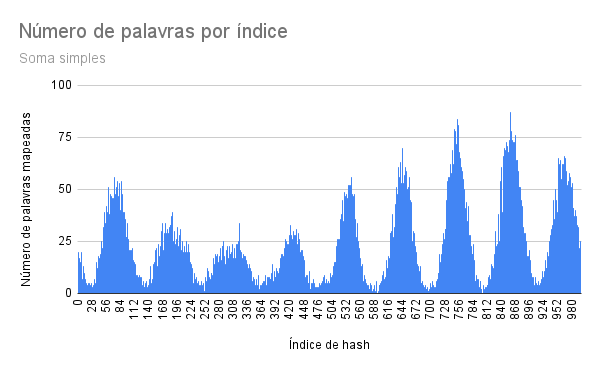
\includegraphics[width=0.9\textwidth]{soma_simples.png}
\caption{Distribuição de palavras distintas por índice da tabela usando a função de hash baseada na soma dos caracteres.}
\end{figure}

\subsubsection*{Resultados com $N = 50000$}

Repetimos o experimento com a função baseada na soma dos caracteres, agora utilizando uma tabela com $N = 50000$ posições. 
Apesar do aumento expressivo no tamanho da tabela, os resultados permaneceram insatisfatórios:

\begin{itemize}
  \item \textbf{48.600 posições} da tabela ficaram completamente vazias;
  \item A maior carga observada em um único índice foi novamente de \textbf{87 palavras distintas};
  \item O número total de colisões foi de \textbf{20.677}, praticamente igual ao observado com $N = 1000$;
  \item Apenas uma pequena faixa inicial da tabela foi efetivamente utilizada -- a maioria dos índices jamais recebeu qualquer palavra.
\end{itemize}

Esse comportamento ocorre porque a função de hash baseada na soma dos caracteres gera valores relativamente baixos: como a maioria das palavras tem entre 4 e 15 letras e utiliza caracteres com códigos entre 97 e 122 (no caso de letras minúsculas), a soma total raramente ultrapassa 1500. 
Com isso, todos os valores de hash produzidos se concentram nos primeiros mil ou dois mil índices da tabela. 
Os demais índices -- mais de 90\% da tabela -- simplesmente não são utilizados. 
Isso evidencia uma das principais falhas dessa função: sua incapacidade de aproveitar o espaço disponível, mesmo quando a tabela é grande.


\subsubsection*{Por que essa função falha?}

Apesar de ser válida como função no sentido técnico (é determinística e retorna um valor inteiro), essa função é inadequada para uso prático em tabelas de dispersão. 
Os principais problemas são:

\begin{itemize}
  \item \textbf{Ignora a ordem dos caracteres:} palavras como \texttt{amor} e \texttt{roma} têm o mesmo valor de hash.
  \item \textbf{Alta redundância linguística:} palavras com estruturas semelhantes (prefixos, sufixos, letras de mesmo valor) tendem a cair nas mesmas posições.
  \item \textbf{Pouca difusão:} pequenas mudanças na entrada resultam em mudanças pequenas no hash.
\end{itemize}

Esse exemplo mostra que a escolha da função de hash tem impacto direto sobre a eficiência da tabela: funções simples demais podem gerar um número elevado de colisões, comprometendo o desempenho das operações básicas.

\subsection*{Função polinomial com base 31}

A segunda função que analisamos é baseada em um cálculo polinomial clássico, que atribui pesos crescentes aos caracteres da string conforme sua posição:
\[
h(s) = (c_0 + 31 \cdot c_1 + 31^2 \cdot c_2 + \dots + 31^{n-1} \cdot c_{n-1}) \bmod N
\]
onde $c_i$ representa o valor numérico do $i$-ésimo caractere. Essa função leva em conta a ordem dos caracteres, o que a torna mais sensível a variações entre palavras diferentes.

\begin{example}
\subsubsection*{Exemplo ilustrativo}

Vamos agora calcular o valor da função de hash polinomial com base 31 para a palavra \texttt{programador}. Essa função considera a ordem dos caracteres e aplica pesos exponenciais:

\[
h(s) = (c_0 + 31 \cdot c_1 + 31^2 \cdot c_2 + \dots + 31^{n-1} \cdot c_{n-1}) \bmod N
\]

Para \texttt{programador}, com $N = 1000$, temos os seguintes valores ASCII:

\begin{center}
\begin{tabular}{c|c|l}
Letra & Código & Peso \\
\hline
p & 112 & $31^0$ = 1 \\
r & 114 & $31^1$ = 31 \\
o & 111 & $31^2$ = 961 \\
g & 103 & $31^3$ = 29.791 \\
r & 114 & $31^4$ = 923.521 \\
a & 97 & $31^5$ = 28.628.151 \\
m & 109 & $31^6$ = 887.472.681 \\
a & 97 & $31^7$ = 27.511.653.111 \\
d & 100 & $31^8$ = 852.861.246.441 \\
o & 111 & $31^9$ = 26.438.698.639.671 \\
r & 114 & $31^{10}$ = 820.599.658.829.801 \\
\end{tabular}
\end{center}

Multiplicamos cada caractere por seu respectivo peso e somamos todos os produtos:

\[
h(\texttt{programador}) = (112 \cdot 1 + 114 \cdot 31 + 111 \cdot 961 + \dots + 114 \cdot 820.599.658.829.801) \bmod 1000
\]

O valor intermediário fica enorme, mas ao aplicar o módulo 1000 em cada etapa (ou no final), obtemos:

\[
h(\texttt{programador}) \equiv 722\ \bmod\ 1000
\]

Esse exemplo mostra como a função polinomial leva em conta tanto os valores dos caracteres quanto sua posição. 
Palavras com os mesmos caracteres em ordens diferentes terão valores distintos, e o efeito exponencial ajuda a dispersar melhor os dados pela tabela.


\end{example}

\subsubsection*{Resultados com $N = 1000$}

Aplicamos essa função ao mesmo conjunto de 22.077 palavras distintas, utilizando uma tabela de tamanho $N = 1000$. Os resultados foram significativamente melhores do que na função baseada na soma:

\begin{itemize}
  \item \textbf{Nenhuma posição} da tabela ficou vazia;
  \item A maior carga observada em um único índice foi de \textbf{38 palavras distintas};
  \item O número total de colisões foi de \textbf{21.077}, substancialmente menor do que o número total de entradas (o que é esperado, dado que $n > N$);
  \item A distribuição dos valores foi mais uniforme, com menos aglomerações extremas.
\end{itemize}

\begin{figure}[h]
\centering
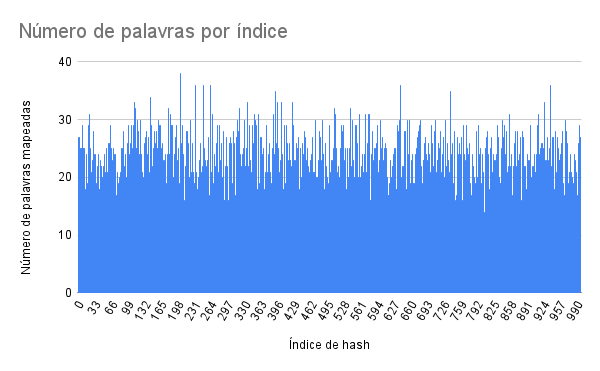
\includegraphics[width=0.9\textwidth]{polinomial.png} % Nome do gráfico gerado
\caption{Distribuição de palavras distintas por índice da tabela usando a função de hash polinomial com base 31.}
\end{figure}

\subsubsection*{Por que essa função funciona melhor?}

Comparada à função da soma, a função polinomial apresenta várias vantagens:

\begin{itemize}
  \item \textbf{Considera a ordem dos caracteres:} isso evita que anagramas gerem o mesmo valor de hash.
  \item \textbf{Maior variação:} o uso de potências introduz um efeito de amplificação, mesmo para pequenas mudanças na string.
  \item \textbf{Distribuição mais equilibrada:} o número de posições ocupadas e a dispersão geral das chaves foram significativamente melhores.
\end{itemize}

Esse experimento mostra que, mesmo com um número de colisões inevitável quando $n \gg N$, uma função de hash bem projetada pode reduzir o impacto dessas colisões ao espalhar melhor os dados pela tabela.

\subsubsection*{Resultados com $N = 50000$}

Repetimos o experimento com a função polinomial base 31 utilizando uma tabela significativamente maior: $N = 50000$.

\begin{itemize}
  \item O número total de colisões foi de apenas \textbf{4.236};
  \item A maior carga observada em um único índice foi de \textbf{5 palavras distintas}.
\end{itemize}

Esses resultados mostram como o aumento do tamanho da tabela reduz drasticamente o número de colisões. 
Embora muitas posições da tabela fiquem vazias -- o que é natural quando $N$ é muito maior que o número de elementos -- as posições ocupadas recebem em geral apenas uma ou duas palavras. 
A distribuição resultante é bastante equilibrada, com poucas colisões e sem pontos de concentração.


